\chapter{پیاده‌سازی و نتایج}

\section{تخمین عمر مفید باقی‌مانده}
در جدول ۵-۱ بخشی از نتایج مربوط به کارتحقیقاتی فالکن و همکاران که مدلی بر پایه ماتع برای تحمین عمر مفید باقی‌مانده وسایل مکانیکی پیشنهاد داده بودند آورده شده است. آن‌ها برای ارزیابی مدل از یک تابع امتیاز که در مقاله‌ای دیگر معرفی شده بود و معیار خطای ریشه میانگین مربعات خطا\LTRfootnote{Rooted Mean Square Error (RMSE} استفاده کرده بودند. هر چه این دو معیار برای یک مدل پایین‌تر باشد آن مدل کاراتر است. 

\begin{table}[!h]
\begin{center}
\caption{نتایج کار تحقیقاتی فالکن و همکاران برای تخمین عمر مفید باقی‌مانده\cite{falcon2020neural}}
\begin{tabular}{r|r|r}
\toprule
\textbf{مدل} & \textbf{امتیاز} & \textbf{ریشه میانگین مربعات خطا}
\\
\hline
\hline
\lr{LSTM} & ۳۳۹ & ۱۶/۱۶
\\
\lr{LSTM} + ماتع & ۲۴۲ & ۱۲/۵۰
\\
\bottomrule
\end{tabular}
\end{center}
\end{table}

همانگونه که مشخص است استفاده از ماتع در کنار \lr{LSTM} منجر به کاهش حدود ۲۲ درصدی خطا شده است.

\section{دسته‌بندی}
در جدول ۵-۲ بخشی از نتایج کار تحقیقاتی ملک‌محمدی و صافی‌اصفهانی آورده شده است. در کار تحقیقاتی آن‌ها با بهبود ماتع و استفاده از الگوریتم ازدحام ذرات مدل دسته‌بند کارایی توسعه داده‌اند. معیار ارزیابی آن‌ها صحت\LTRfootnote{Accuracy} بوده است. برای مجموعه‌داده دسته‌بندی هم از چهار مجموعه‌داده مطرح در این حوزه استفاده کردند. نهایتا برای مدل از مدل‌های دسته‌بند بردار ماشین پشتیبان \LTRfootnote{Support Vector Machine(SVM}، \lr{k}-نزدیک‌ترین همسایه \LTRfootnote{K-Nearest Neighbour (KNN)}، بیز ساده‌لوحانه\LTRfootnote{Naive Bayes}، \lr{LSTM}، ماتع استاندارد، کامپیوتر عصبی متمایز\LTRfootnote{Differentiable Neural Computer (DNC} و نهایتا ماتع با الگوریتم ازدحام ذرات که روش پیشنهادی آن‌ها بود استفاده شده است.\cite{faradonbe2020classifier} لازم به ذکر است کامپیوتر عصبی متمایز نیز یکی از افزونه‌های مانع است که در این گزارش به آن پرداخته نشده است. نتایج در جدول ۵-۲ آورده شده است. 
\\

\begin{table}[!h]
\begin{center}
\caption{نتایج کار تحقیقاتی ملک‌محمدی و صافی‌اصفهانی برای دسته‌بندی \cite{faradonbe2020classifier}}
\begin{tabular}{p{1.7cm}||p{1.1cm}|p{1.1cm}|p{1.1cm}|p{1.1cm}|p{1.1cm}||p{1.1cm}|p{1.1cm}|p{1.1cm}}
\toprule
\textbf{مجموعه داده} & \textbf{ماشین پشتیبان} & \textbf{\lr{k}-نزدیک ترین همسایه} & \textbf{بیز ساده لوحانه} & \textbf{درخت تصمیم} & \textbf{\lr{LSTM}} & \textbf{ماتع} & \textbf{کامپیوتر عصبی متمایز} & \textbf{ماتع + الگوریتم ازدحام ذرات}
\\
\hline
\hline
\lr{MNIST} & 94/16 & 96/9 & 56/15 & 65/40 & 96/48 & 96/96 & 99/12 & 99/73
\\
\lr{ORL} & 84/68 & 92/5 & 77/25 & 88/5 & 94/2 & 95/11 & 97/21 & 97/9
\\
\lr{\lr{Leter}} & 84/11 & 89/81 & 93/21 & 83/6 & 95/5 & 96/01 & 98/16 & 99/02 
\\
\lr{Ionosphere} & 80/3 & 77/78 & 82/62 & 84/5 & 91/16 & 93/41 & 96/02 & 97/1
\\
\bottomrule

\end{tabular}
\end{center}
\end{table}

همانطور که از نتایج جدول ۵-۲ بر می‌آید بهترین دقت‌های برای سه مدلی است که بر پایه ماتع طراحی شده‌اند. این‌ها نشان از کارایی ماتع و افزونه‌های آن برای کاربرد دسته‌بندی است.

\section{ردیابی دانش}
شکل ۵-۱ شامل بخشی از نتایج آزمایشات انجام‌شده ژائو و همکاران است. آن‌ها برای ارزیابی از معیار صحت و ناحیه زیر نمودار\LTRfootnote{Area Under Curve (AUC)} استفاده کرده‌اند. مدل رقیب هم شبکه \lr{LSTM} بدون ماتع متوجه است. با توجه به آنکه مدل پیشنهادی آنان برای حل مشکل شروع سرد در حوزه ردیابی دانش ارائه شده است سه سناریو مرتبط با این وضعیت طراحی کرده‌اند:
\begin{enumerate}
\item سناریو اول: دانشجو کم
\item سناریو دوم: دنباله‌های یادگیری فعالیت کوتاه
\item سناریو سوم: هم دانشجو کم و هم دنباله‌های یادگیری فعالیت کوتاه
\end{enumerate} 

\begin{figure}[!h]
\begin{center}
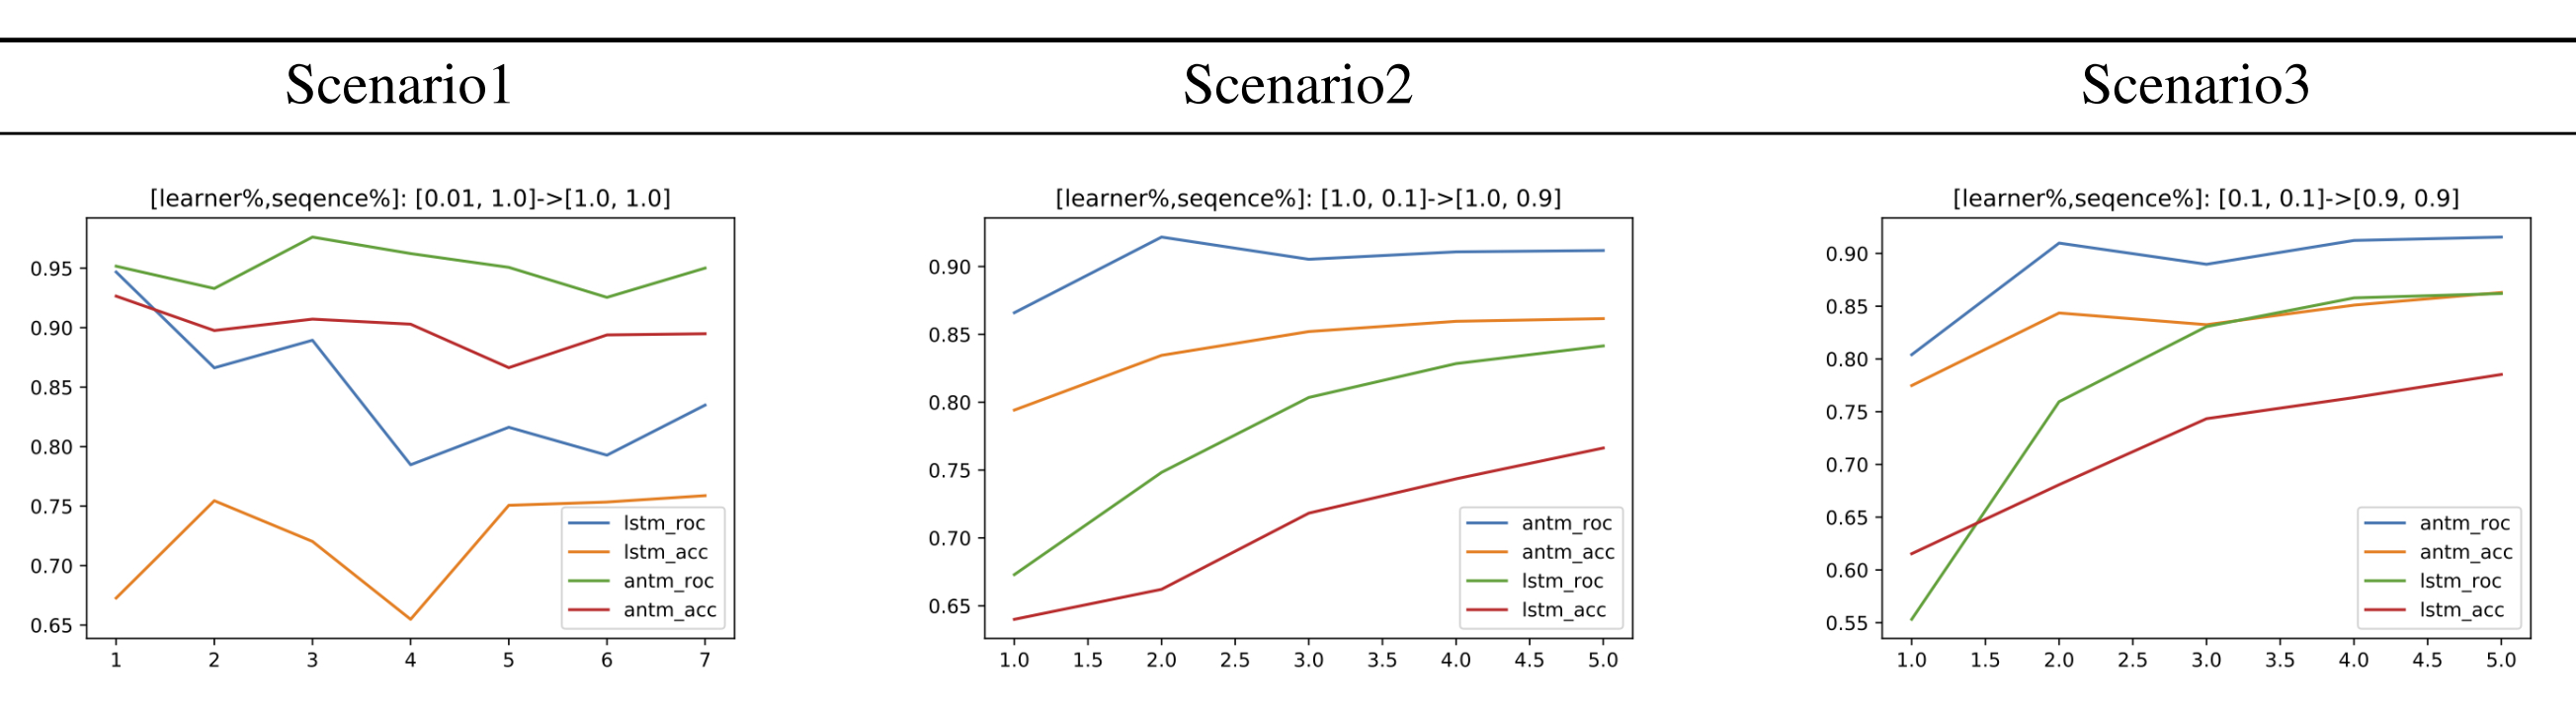
\includegraphics[height=4cm]{ANTM-Results.png}
\end{center}
\caption{نتایج کار تحقیقاتی ژائو و همکاران برای ردیابی دانش\cite{zhao2020cold}}
\medskip
\small

باتوجه به شکل ۵-۱ می‌توان دید که ماتع متوجه به عنوان یکی دیگر از افزونه‌های ماتع توانسته بهبودی برای شروع سرد در کاربرد ردیابی دانش ارائه دهد.

\end{figure}
